% Three prescribed groups of slots illustrate projection onto a simple graph.
% Two groups yield overlapping triangles. The repeated a in the third group
% contributes neither a loop nor a second copy of the already present edge ab.
\begingroup
\definecolor{motifteal}{RGB}{33,112,117}
\definecolor{slotgray}{RGB}{105,113,118}
\definecolor{slotorange}{RGB}{182,112,49}
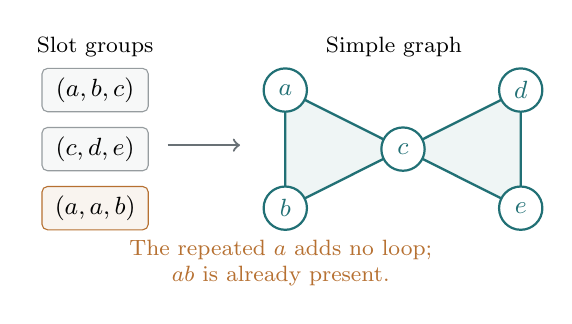
\begin{tikzpicture}[
  x=1.15cm, y=1cm,
  vertex/.style={circle, minimum size=5.5mm, inner sep=0pt, font=\small,
    draw=motifteal, fill=white, text=motifteal, line width=0.8pt},
  slot group/.style={rectangle, rounded corners=2pt, minimum width=1.35cm,
    minimum height=5.5mm, inner sep=3pt, font=\small,
    draw=slotgray!70, fill=slotgray!5},
  edge/.style={draw=motifteal, line width=0.85pt}
]
  \node[font=\footnotesize] at (0,1.55) {Slot groups};
  \node[slot group] at (0,1) {$(a,b,c)$};
  \node[slot group] at (0,0.25) {$(c,d,e)$};
  \node[slot group, draw=slotorange, fill=slotorange!8] at (0,-0.5)
    {$(a,a,b)$};
  \draw[->, draw=slotgray, line width=0.8pt] (0.8,0.3)--(1.6,0.3);
  \node[font=\footnotesize] at (3.3,1.55) {Simple graph};
  % The resulting edge set is {ab,ac,bc,cd,ce,de}; c is shared.
  \coordinate (a) at (2.1,1);
  \coordinate (b) at (2.1,-0.5);
  \coordinate (c) at (3.4,0.25);
  \coordinate (d) at (4.7,1);
  \coordinate (e) at (4.7,-0.5);
  \fill[motifteal!7] (a)--(b)--(c)--cycle;
  \fill[motifteal!7] (c)--(d)--(e)--cycle;
  \draw[edge] (a)--(b)--(c)--cycle (c)--(d)--(e)--cycle;
  \foreach \v in {a,b,c,d,e} \node[vertex] at (\v) {$\v$};
  \node[font=\footnotesize, text=slotorange, align=center] at (2.05,-1.2)
    {The repeated $a$ adds no loop;\\$ab$ is already present.};
\end{tikzpicture}
\endgroup
